\chapter{Technical Background}
\label{sec:state}

% Hier werden zwei wesentliche Aufgaben erledigt:

% 1. Der Leser muß alles beigebracht bekommen, was er zum Verständnis
% der späteren Kapitel braucht. Insbesondere sind in unserem Fach die
% Systemvoraussetzungen zu klären, die man später benutzt. Zulässig ist
% auch, daß man hier auf Tutorials oder Ähnliches verweist, die hier auf
% dem Netz zugänglich sind.

% 2. Es muß klar werden, was anderswo zu diesem Problem gearbeitet
% wird. Insbesondere sollen natürlich die Lücken der anderen klar
% werden. Warum ist die eigene Arbeit, der eigene Ansatz wichtig, um
% hier den Stand der Technik weiterzubringen? Dieses Kapitel wird von
% vielen Lesern übergangen (nicht aber vom Gutachter ;-), auch später
% bei Veröffentlichungen ist "Related Work" eine wichtige Sache.

% Viele Leser stellen dann später fest, daß sie einige der Grundlagen
% doch brauchen und blättern zurück. Deshalb ist es gut,
% Rückwärtsverweise in späteren Kapiteln zu haben, und zwar so, daß man
% die Abschnitte, auf die verwiesen wird, auch für sich lesen
% kann. Diese Kapitel kann relativ lang werden, je größer der Kontext
% der Arbeit, desto länger. Es lohnt sich auch! Den Text kann man unter
% Umständen wiederverwenden, indem man ihn als "Tutorial" zu einem
% Gebiet auch dem Netz zugänglich macht.

% Dadurch gewinnt man manchmal wertvolle Hinweise von Kollegen. Dieses
% Kapitel wird in der Regel zuerst geschrieben und ist das Einfachste
% (oder das Schwerste weil erste).

%\ldots state of the art \ldots

%\todo{write state}
This chapter provides background knowledge of all the content and topics covered in the thesis. This thesis presumes that the reader is 
already aware of the basic concepts of operating system, kubernetes\cite*{k8s}, and confidential computing. Nevertheless, it offers a brief overview of some essential terms and 
concepts to help the reader better understand the later chapters. For a short rundown of associate terminology, please check the glossary on 
this page.
\todo{add glossary page nummber}
\section{Kubernetes}
\begin{figure}[H]
    \centering
    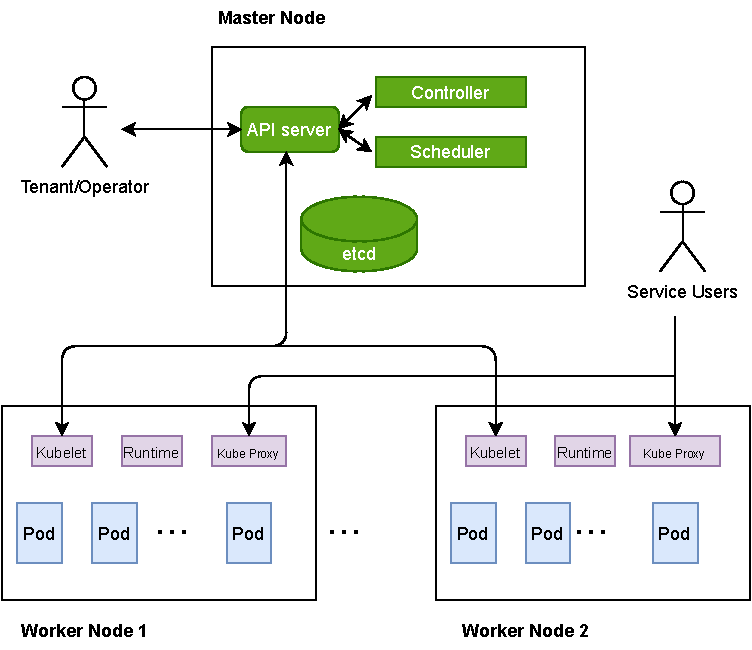
\includegraphics[width=0.8\textwidth]{images/k8s_arch.pdf}
    \caption[k8s arch]{k8s arch}
    \label{fig:k8s_arch}
  \end{figure}
\todo{add description for k8s architectural diagram}

Kubernetes\cite*{k8s} is a portable, scalable open-source platform for managing and orchestrating containerized workloads. Kubernetes emerged because, in the context of the rise of cloud computing, more and more applications are being deployed to the cloud, 
and cloud operators need an automated tool to manage thousands of containers. Kubernetes provides operators with a framework for running cloud-native applications\cite*{KRATZKE20171} in both elastically and resiliently manner. 
It undertakes application scaling and failover and offers a variety of deployment models.

Kubernetes also introduces the concept of pod. In a cluster, a pod, which consists of one or more containers sharing network and storage resources, is the smallest deployment unit managed by Kubernetes. It has a unique cluster-IP address, and the containers within it 
can communicate with each other through the localhost. In addition, Kubernetes support different isolation levels of pods. With the runtime class keyword, clients can choose to deploy pods based on Linux namespace and cgroup for better performance, 
or hardware virtualization for better security\cite*{k8s_runtime_class}.


\subsection{Kubernetes architecture}
From an architectural point of view, a k8s cluster consists of at least one master node and several worker nodes. A node can be a physical or virtual machine. The master node consists of a series of control plane components that make global decisions 
about the cluster, including scheduling, detecting, and responding to cluster events, for example, dynamically adjusting the number of 
pods in an application based on resource utilization. As shown in figure~\ref{fig:k8s_arch}, these control plane components include the apiserver, controller, scheduler, and ectd\cite*{k8s}. Apiserver provides the kubernetes control plane with an 
interface to control and manage the cluster. Specifically, it can be used to receive and authenticate requests from users and other components of the cluster, and update the corresponding API objects that include services pods, and replication 
controllers. Controller is a control loop that continuously monitors the state of the cluster and attempts to move the current state of the cluster to the desired state. For example, the Node controller is responsible for monitoring the state 
of each node and responding accordingly when a node crash. Scheduler continuously search undeployed pods and deploys them to an appropriate worker node. Factors that influence scheduling decisions are resource requirements, 
hardware/software/policy constraints, affinity, data locality, and inter-workload interference. The etcd is a distributed, highly available key-value store for storing cluster level data.


Each worker node runs and maintains the pods. It consists of three main components, kube-proxy, kubelet, and container high/low-level runtime. The kube-proxy running on each node implements part of the Kubernetes service and maintains network rules 
on each node, which allows network access to pods from both within and outside the cluster. As for kubelet, it acts as an agent, listening for requests/commands from the master and calling other services located on the same node to fulfill the 
request. In the case of container/image management-related requests, it makes a call to a host-chosen high-level container runtime, like containerd\cite*{containerd} or ciro\cite*{cri-o}. These high-level container runtimes are responsible for managing the container lifecycle 
and images, and delegate the actual creation/deletion of pod/containers to lower-level container runtimes or so-called shim process. Examples of low level container runtime include kata, qvisor, quark, runc, etc,.


\subsection{OCI Runtime Specification and Low level container runtimes}
There are various low-level container runtimes available in the market to meet the different needs of users for container security and performance. For example, security-sensitive customers can use the kata runtime to create virtual machine-based 
containers, which provides 2 layers of isolation. However, these container runtime implementations can break container portability and compatibility between container runtimes.

To address this issue, the Open Container Initiative has proposed the OCI runtime specification which outlines how a low levle container runtime creates and runs containers based on "file system packages" and how to manage the lifecycle of containers.

The "file system bundle" holds the container root file system and the metadata needed to create and run containers. This metadata includes the following information: metadata related to the application process, such as process environment variables 
and process arguments, metadata defining the container root file system, and mount information, which specifies the additional file systems that should be mounted to the container root file system by low level container runtime. Besides, for Linux 
platforms, this metadata may also contain configuration for process security and resource limits, such as rlimits, AppArmor, and SELinux labels, as well as hooks, which enable one to extend the functionality of a low-level runtime by hooking 
executables into the container lifecycle. This is shown in the following state diagram.

\begin{figure}[tbp]
  \centering
  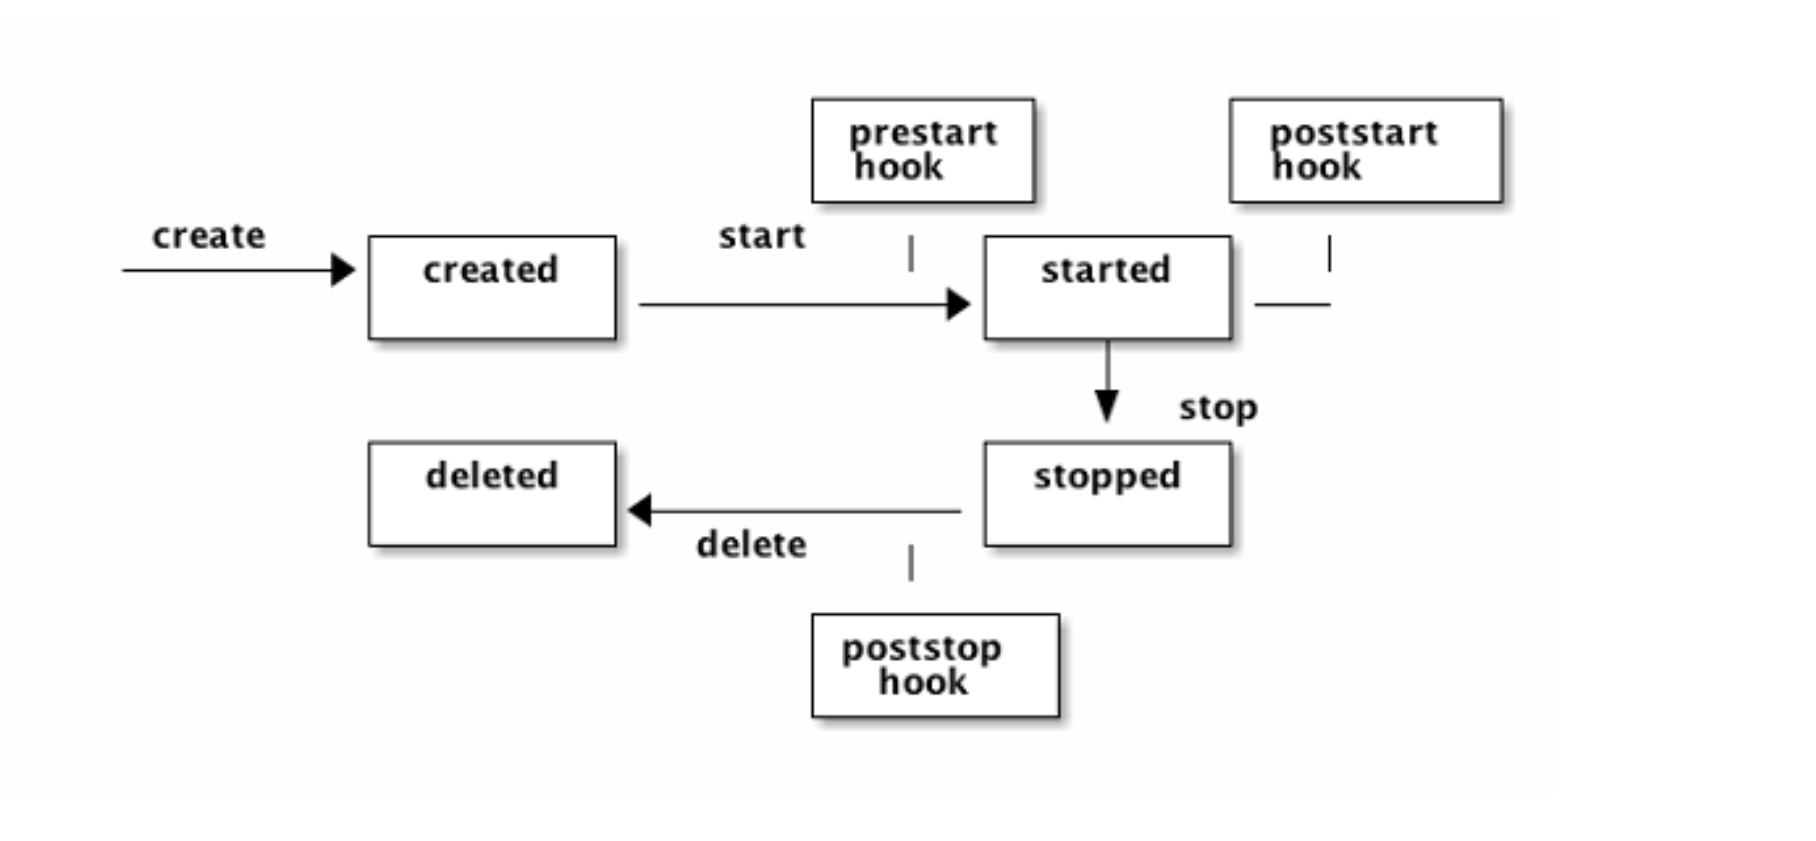
\includegraphics[width=0.8\textwidth]{images/Container_Lifecycle_state}
  \caption[Short description]{container lifecycle and hooks. Image taken from \url{https://www.alibabacloud.com/blog/open-container-initiative-oci-specifications_594397}}
  \label{fig:Container_Lifecycle_state}
\end{figure}
How does the OCI runtime work in practice? Upon receiving the "container creation request", high-level container runtime configures container network namespaces and preprocess container images during the container build process. This includes 
pulling the image from remote, unpacking the image, 
creating a "file system bundle" and forwarding it to an OCI-compatible low-level container runtime. Since the low-level container runtime is implemented following the OCI runtime specification,  it has the ability to set up the environment and run 
the container based on a "file system bundle ". In this way,  we prevent fragmentation caused by different low-level container runtime implementations.  In other words, the OCI runtime specification greatly enhances interoperability between the 
high-level container runtime and various low-level container runtime implementations.



\subsection{Open Standards (CRI\cite*{cri-interface}, Shim V2 API, OCI\cite*{oci-spec}) makes Kubernetes more extensible}
\subsubsection{Container Runtime Interface (CRI)}
Nowadays, there are various high-level container runtimes on the market. The most popular of them are CRI-O\cite*{cri-o}, and Containerd\cite*{containerd}. However, different implementations of high-level container runtimes increase 
the effort required to integrate them into kubelet. This problem was solved when k8s proposed the Container Runtime Interface (CRI)\cite*{cri-interface}. It consists of two gRPC service interfaces, the ImageService 
interface and the RuntimeServec. As showed in code snippet \Nameref{CRI_INTERFACE}, the ImageService interface defines the endpoints for managing images, while the RuntimeServec interface includes endpoints for managing containers and pods. 
\begin{lstlisting}[language=rust, basicstyle=\small, caption={Container Runtime Interface (CRI)}, title={Container Runtime Interface (CRI)}, label={CRI_INTERFACE}]
  // ImageService defines the public APIs for managing images.
  service ImageService {
      rpc ListImages(ListImagesRequest) 
      rpc ImageStatus(ImageStatusRequest)
      rpc PullImage(PullImageRequest)
      rpc RemoveImage(RemoveImageRequest)
      rpc ImageFsInfo(ImageFsInfoRequest)
  }

  // Runtime service defines the public APIs for remote container runtimes
  service RuntimeService {
      rpc Version(VersionRequest)
      rpc RunPodSandbox(RunPodSandboxRequest)
      rpc StopPodSandbox(StopPodSandboxRequest)
      rpc RemovePodSandbox(RemovePodSandboxRequest)
      rpc PodSandboxStatus(PodSandboxStatusRequest)
      rpc ListPodSandbox(ListPodSandboxRequest)
      rpc CreateContainer(CreateContainerRequest)
      rpc StartContainer(StartContainerRequest)
      rpc StopContainer(StopContainerRequest)
      rpc RemoveContainer(RemoveContainerRequest)
      rpc ListContainers(ListContainersRequest)
      rpc ContainerStatus(ContainerStatusRequest)
      rpc UpdateContainerResources(UpdateContainerResourcesRequest)
      rpc ReopenContainerLog(ReopenContainerLogRequest)
      rpc ExecSync(ExecSyncRequest)
      rpc Exec(ExecRequest)
      rpc Attach(AttachRequest)
      rpc PortForward(PortForwardRequest)
      rpc ContainerStats(ContainerStatsRequest)
      rpc ListContainerStats(ListContainerStatsRequest)
      rpc PodSandboxStats(PodSandboxStatsRequest)
      rpc ListPodSandboxStats(ListPodSandboxStatsRequest)
      rpc UpdateRuntimeConfig(UpdateRuntimeConfigRequest) 
      rpc Status(StatusRequest)
  }
\end{lstlisting}

Any high-level runtime that wants to integrate into the Kubernetes ecosystem must implement the endpoints defined in the CRI. Thus, it acts as a communication protocol between the kubelet and the 
high-level container runtime allowing the kubelet to access the services provided by any container runtime that implements the CRI interface. Through the CRI interface,  kubelet breaks the dependency with a specific 
high-level container runtime, thus greatly improving the scalability of Kubernetes.

\subsubsection{Shim V2 API}
There are different low level container runtimes on the market that can meet various customer needs, namely security-oriented container runtimes such as kata and quark, and performance-oriented runtimes including Runc (containers for the Linux kernel). 
However, this can bring great integration overhead for high-level container runtime developers if they want to support these lower-level container runtimes. For example, if the contained wants to run both kata-based and quark-based containers, 
the containerd developer has to write two integration patches and make sure they are compatible to the containerd code base. Followed the idea of CRI, the community addressed this problem by defining the shim interface, which aims to 
decouple the low level runtime from the high-level runtime and prevent any code invasion into the high-level container runtime during the integration process.
 %or \small or \footnotesize etc. \tiny
 \begin{lstlisting}[language=rust, basicstyle=\small, caption={Shim V2 Api}, title={Shim V2 Api}, label={shim_v2}]
  pub trait Task {
      fn state(&self, _ctx: &::ttrpc::TtrpcContext, _req: super::shim::StateRequest)
      fn create(&self, _ctx: &::ttrpc::TtrpcContext, _req: super::shim::CreateTaskRequest)
      fn start(&self, _ctx: &::ttrpc::TtrpcContext, _req: super::shim::StartRequest)
      fn delete(&self, _ctx: &::ttrpc::TtrpcContext, _req: super::shim::DeleteRequest)
      fn pids(&self, _ctx: &::ttrpc::TtrpcContext, _req: super::shim::PidsRequest)
      fn pause(&self, _ctx: &::ttrpc::TtrpcContext, _req: super::shim::PauseRequest)
      fn resume(&self, _ctx: &::ttrpc::TtrpcContext, _req: super::shim::ResumeRequest)
      fn checkpoint(&self, _ctx: &::ttrpc::TtrpcContext, _req: super::shim::CheckpointTaskRequest)
      fn kill(&self, _ctx: &::ttrpc::TtrpcContext, _req: super::shim::KillRequest)
      fn exec(&self, _ctx: &::ttrpc::TtrpcContext, _req: super::shim::ExecProcessRequest)
      fn resize_pty(&self, _ctx: &::ttrpc::TtrpcContext, _req: super::shim::ResizePtyRequest)
      fn close_io(&self, _ctx: &::ttrpc::TtrpcContext, _req: super::shim::CloseIORequest)
      fn update(&self, _ctx: &::ttrpc::TtrpcContext, _req: super::shim::UpdateTaskRequest)
      fn wait(&self, _ctx: &::ttrpc::TtrpcContext, _req: super::shim::WaitRequest)
      fn stats(&self, _ctx: &::ttrpc::TtrpcContext, _req: super::shim::StatsRequest)
      fn connect(&self, _ctx: &::ttrpc::TtrpcContext, _req: super::shim::ConnectRequest)
      fn shutdown(&self, _ctx: &::ttrpc::TtrpcContext, _req: super::shim::ShutdownRequest)
  }
  \end{lstlisting}
  
In the context of containerd, this shim interface is called the shim v2 API. As depicted in code snippet \nameref{shim_v2}, it is an api that contains multiple ttrpc endpoints. These endpoints specify the requirements for the low level container runtime 
to integrate with containerd. To this end, the low-level runtime should implement these endpoints in order to run with containerd.


\subsubsection{CRI and Shim V2 Api in Practice}
In this section, we present you with a concrete example of how containerd uses CRI and Shim V2 Api and 
various components to create a container. The following diagram shows how containerd works with a kubelet to create an LXC-based container, where containerd implements the cri interface 
through the cri plugin and employs the shim v2 api to notify the shim process to create a container.

\begin{figure}[H]
    \centering
    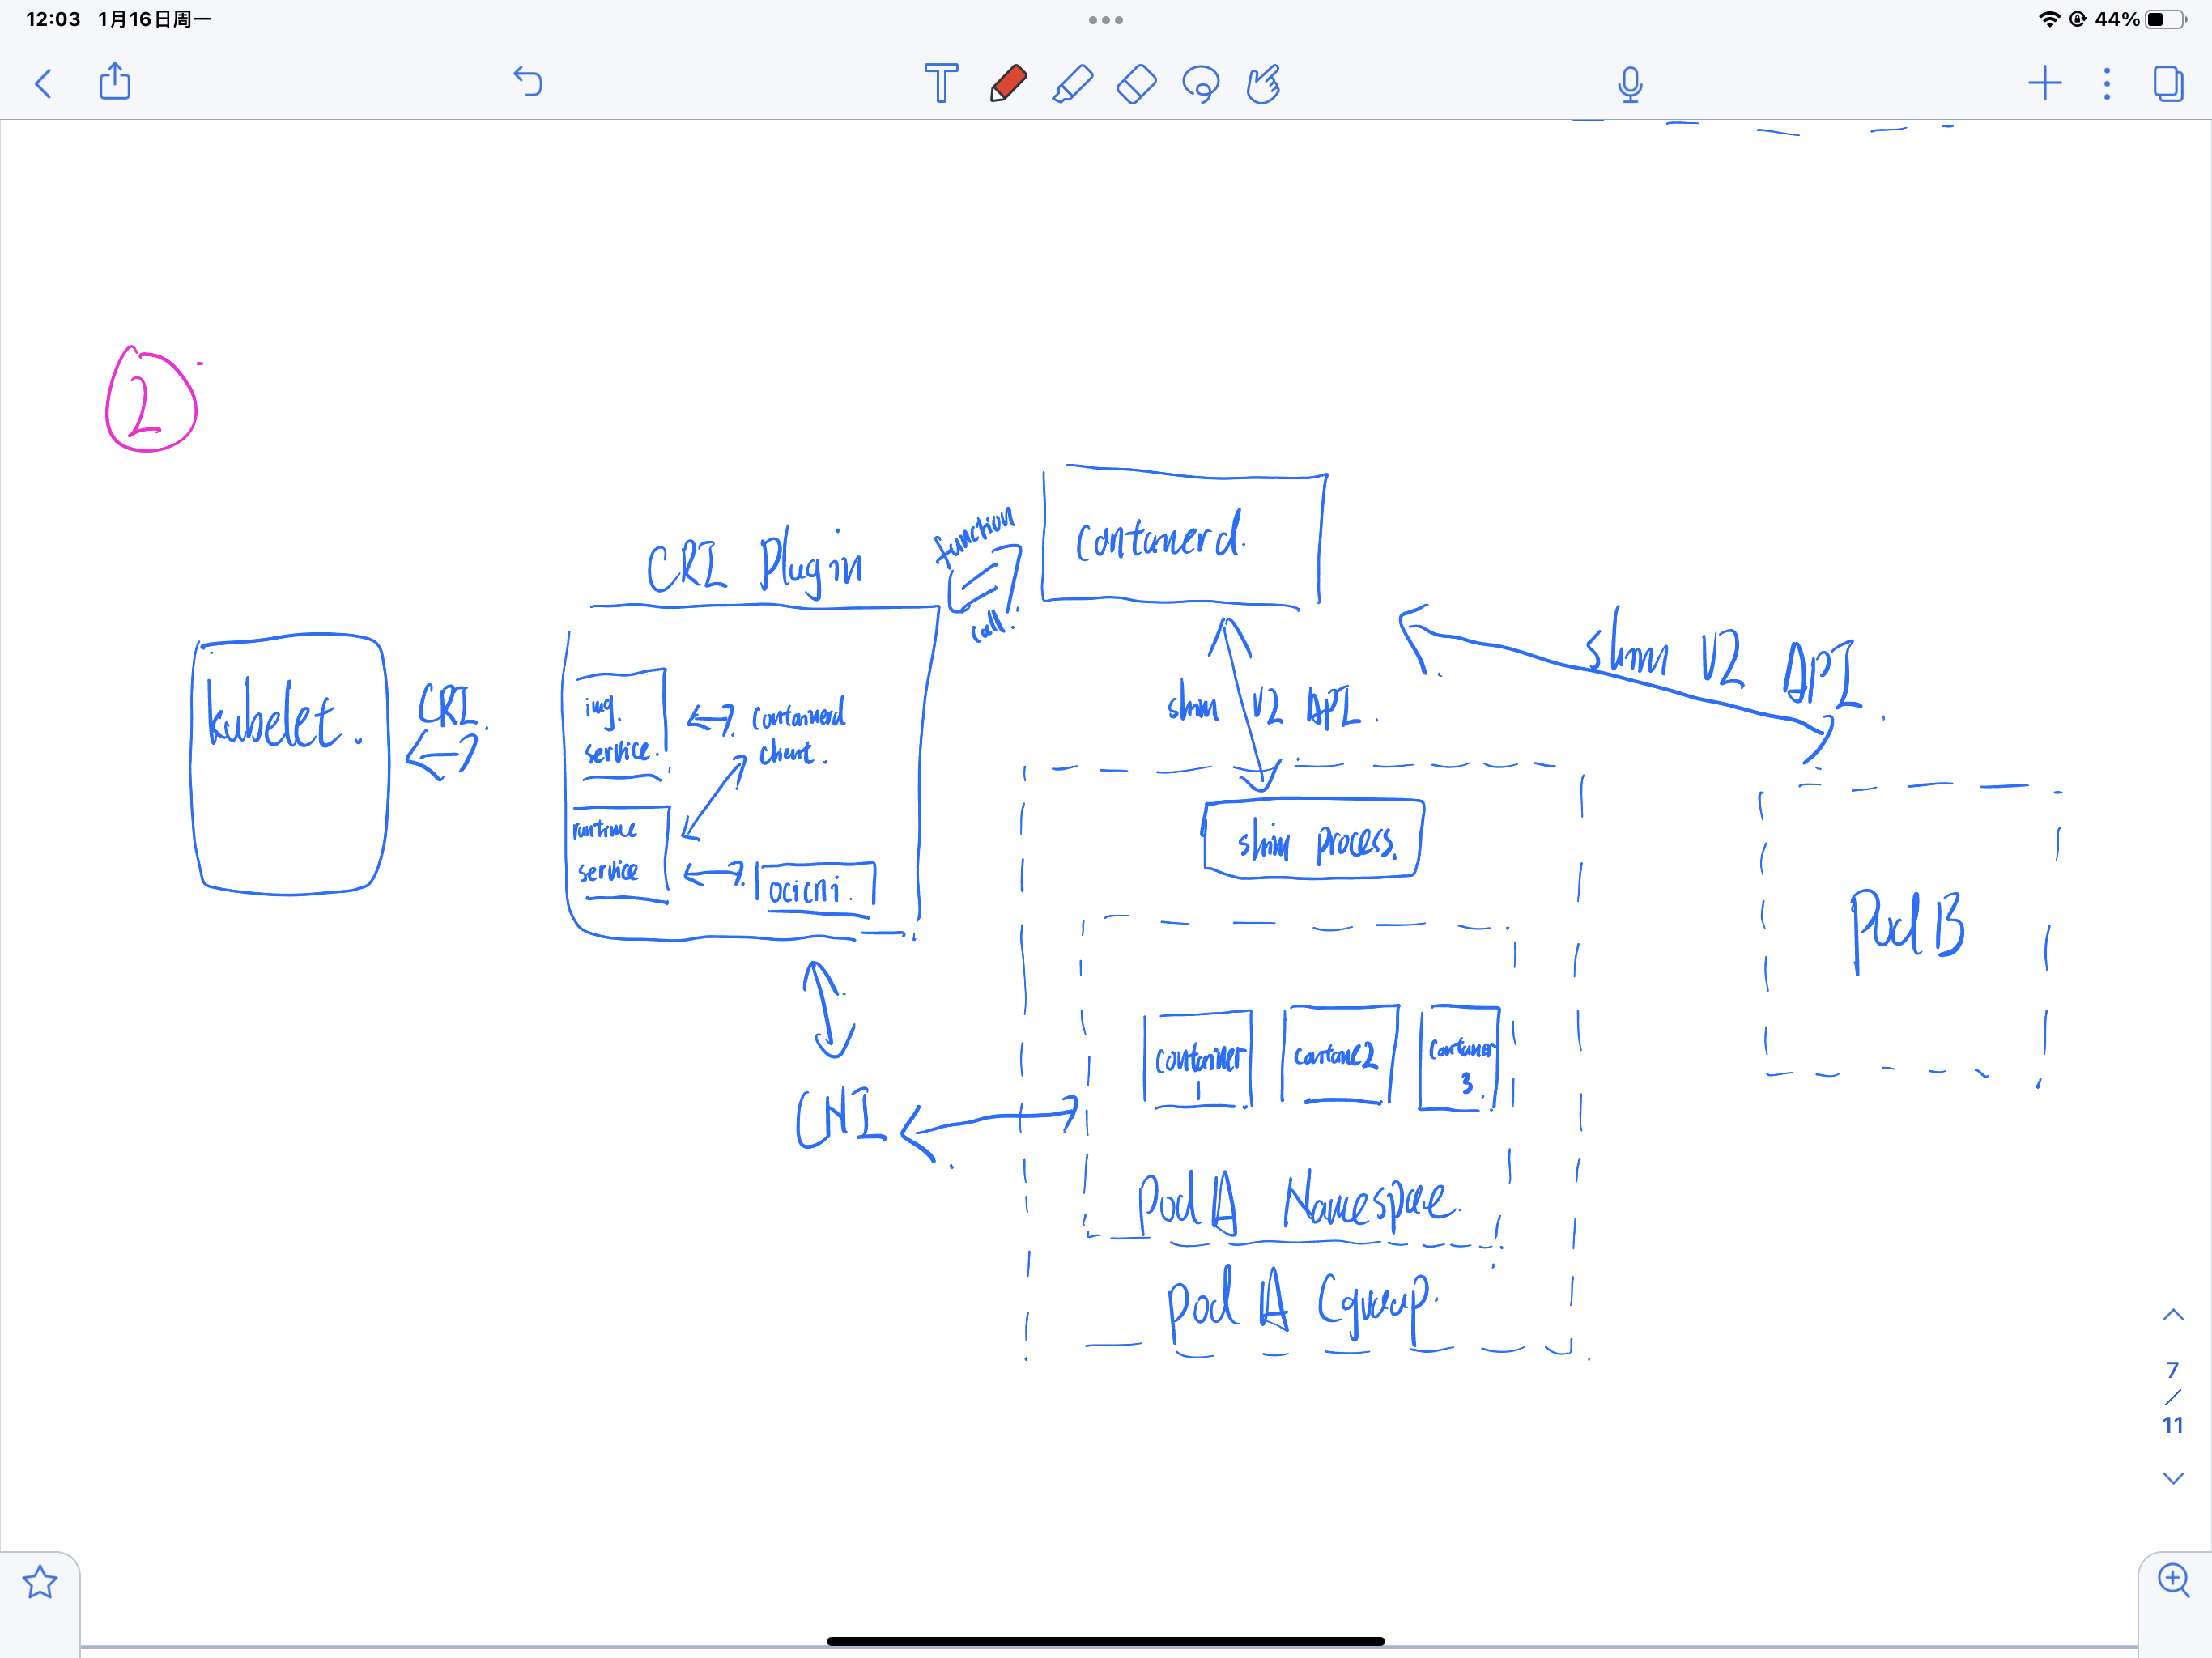
\includegraphics[width=0.8\textwidth]{images/IMG_4417.PNG}
    \caption[Kubelet Workflow]{Kubelet Workflow}
    \label{fig:Kubelet}
\end{figure}
Upon receipt of a ’create container in a new pod’ request from master node, kubelet  creates a pod by calling the cri plugin through the CRI Runtime Services API. 
Cri plugin first creates network namespace for the pod ,and configured the namespace using CNI (Container Network Interface), Then, the cri plugin start a shim process that implements the shim v2 api by calling the containerd's functions.
After the a shim process is launch properly, The cri plugin instructs the shim to create a pod through create and start ttrpc endpoints defined in the shim v2 api. Specifically, This include creating a special pause container as the the sandbox/root container in the pod's cgroups and namespace.
Once the pod is running, kubelet invokes the cri plug-in again through the CRI Image Service API to pull the application container's image. If there is no image on the local registry, the cri plugin further make use of containerd to pull the image from remote
The final step is to crate and start application container inside the pod,  This operation is done by kubelet that sends create and start cmd to the cri plugin  using the CRI Runtime Services API. Cri plugin in turn forwards those cmds to shim process, which
loads the container root filesystem from a subdirectory of containerd and creates the container in the pod. After these steps, the application container is created and runs in this pod.
% \begin{itemize}
%     \item Kubelet creates a pod by calling the cri plugin through the CRI Runtime Services API.
%     \item The cri plug-in create network namespace for the pod, then employ the CNI (Container Network Interface) to configure it;
%     \item The cri plugin calls the containerd's function to start a shim process that implements the shim v2 api.
%     \item The cri plugin then issues the create and start pod command to the shim process through the shim api, which creates a special pause container as the the sandbox container in the pod's cgroups and namespace.
%     \item Kubelet then invokes the cri plug-in through the CRI Image Service API to pull the image for application container.
%     \item If there is no image on the local registry, the cri plugin further make use of containerd to pull the image from remote
%     \item Kubelet then contacts the cri plugin by using the CRI Runtime Services API to create and launch the application container inside the pod. inside the pod using the pulled application container image;
%     \item cri plugin in turn forwards those cmds to shim process via shim v2 api.
%     \item The shim process finally loads the container root filesystem from a subdirectory of containerd and creates the container in the pod. After these steps, the application container is created and runs in this pod.
% \end{itemize}




% \subsection{Open Standards (CRI\cite*{cri-interface}, OCI\cite*{oci-spec}) makes Kubernetes more extensible}

% CRI introduces an abstraction layer that empowers kubelet to work with a diverse range of container runtimes without the need to modify cluster components. It defines the requirements of the 
% orchestration system regarding the container runtime and decouples the container runtime from the kubelet source code, which dramatically reduces the effort involved in integrating container 
% runtimes into k8s\cite*{cri-interface}.

% \todo{add long description for cri overview and k8s with oci cri figure}
% \begin{figure}[H]
%     \centering
%     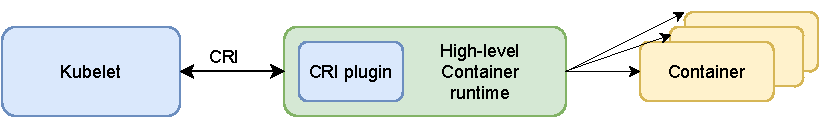
\includegraphics[width=0.8\textwidth]{images/cri_overviwe.pdf}
%     \caption[cri overview]{cri overview}
%     \label{fig:cri_overviwe}
%   \end{figure}


% Figure ~\ref{fig:cri_overviwe} shows the overview of CRI. kubelet communicates with the high-level container runtime via sockets, where the high-level container runtime implements a CRI plugin as a socket server according to the CRI 
% requirements. The socket server provides two primary services to kubelet, namely ImageService and RuntimeService. The ImageService offers kubelet services such as pulling images from remote and 
% inspecting and deleting images managed by the container runtime. The RuntimeService, on the other hand, enables the kubelet to manage the container and sandbox lifecycle 
% (RunPodSandbox /StopPodSandbox/RemovePodSandbox/PodSandboxStatus/CreateContainer/StartContainer/StopContainer, etc.) 
% and interact with containers (attach/port-forward/exec)\cite*{cri-interface}.

% \begin{figure}[H]
%     \centering
%     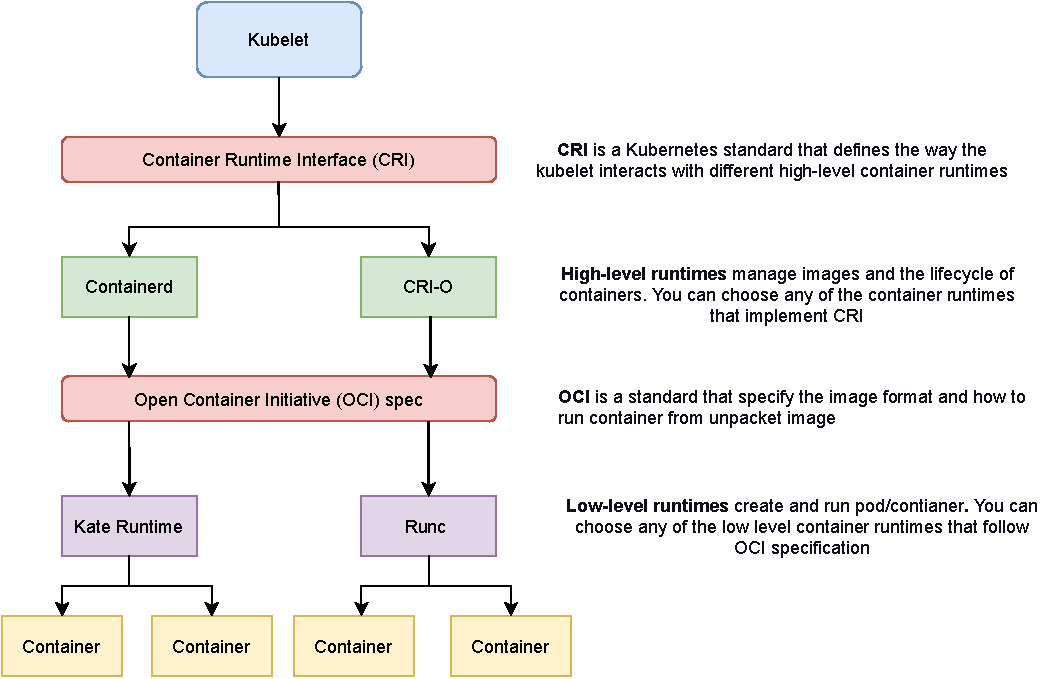
\includegraphics[width=0.8\textwidth]{images/k8s_with_oci_cri.pdf}
%     \caption[k8s with oci cri]{k8s with oci cri}
%     \label{fig:k8s_with_oci_cri}
% \end{figure}
% \todo{add long description for  k8s with oci cri figure}
% In comparison to CRI, which facilitates easy interaction between kubelet and the various high-level container runtimes that manage the image and container lifecycle, the OCI runtime 
% specification\cite*{oci-runtime-spec} defines how low-level container runtimes create and run containers. Typical low-level runtimes are mainly classified as native runtime 
% (runc\cite*{runc}, railcar\cite*{railcar}, Crun\cite*{runc}, rkt\cite*{rkt}) , and Sandboxed-virtualized runtimes (kata runtime\cite*{Kata-Containers}, quark runtime\cite*{quark}, gvisor runtime\cite*{gvisor}, etc.). 
% We refer the readers to \cite*{Runtime-Comparison} for a comprehensive comparison of these container runtimes. Figure~\ref{fig:k8s_with_oci_cri} summarizes how Kubernetes manages containers through the CRI/OCI interface and a variety of high/low-level container runtimes.

% \subsection{Loging}

\section{QUARK CONTAINER}
This section gives a high-level overview of the Quark container\cite*{quark} by introducing its main components and explaining how the guest (Qkenel) communicates with the 
VMM (Qvisor) and host kernel using Hcall ,Qcall, and Ucall, respectively. This explanation is necessary for a better understanding of Chapter 4.

Quark Container is an OCI-compatible container runtime\cite*{oci-runtime-spec}  designed to provide the "security of a virtual machine" while offering the "speed of a 
container\cite*{speed_secure_container_slogen}." It uses KVM hypervisor to launch a virtual machine with a library operating system (Qkernel) written in rust to run containers. 
This container inside VM architecture offers defense in depth. Therefore, a rogue containerized program exploiting a qkernel vulnerability only gains access to qvisor, 
a restricted user process.
Compared to other sandboxed container runtimes, e.g., kata\cite*{Kata-Containers} and gvisor\cite*{gvisor}, using Qkernel as the guest operating system eliminates unnecessary code, 
resulting in a smaller footprint, a faster startup, less overhead, and ensuring the same level of isolation and security for containers\cite*{quark_performance_report}.
\subsection{Architecture}
\begin{figure}[H]
    \centering
    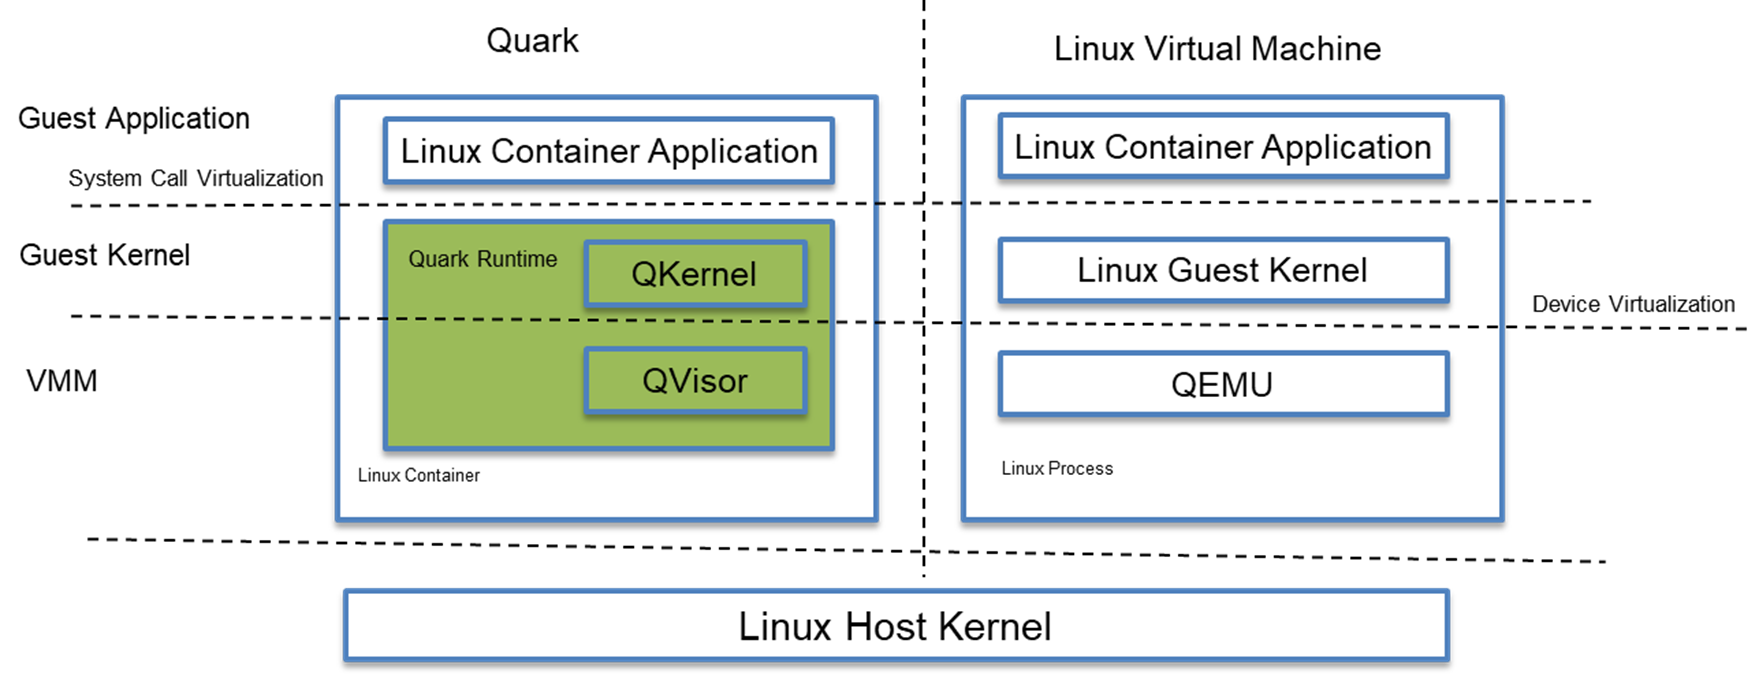
\includegraphics[width=0.8\textwidth]{images/quark_design.png}
    \caption[quark design]{quark design}
    \label{fig:quark_design}
\end{figure}
\todo{add long description for quark design}

In Figure ~\ref{fig:quark_design}, we can see the architecture comparison between Quark-based and Linux virtual machines. The Quark-based virtual machine is shown on the left. This virtual machine consists of Qvisor, 
Qkernel, and several containerized applications. Corresponding to qemu in a Linux virtual machine, qvisor is a virtual machine manager that uses KVM to create and manage the qkernel-based micro VM. 
The qkernel and the containerized applications comprise a virtual machine, where the qkernel serves as the guest operating system and applications run as processes in the guest user space. Unlike 
the Linux guest kernel, qkernel is an ultra-lightweight kernel that contains only necessary code. Furthermore, it implements essential operating system components, such as process management, 
memory management, file system, and network system. Thus, the qkernel, like a macro kernel, provides services to the running program. The user program, in turn, accesses these services via guest 
system calls. i.e., X86-64 SysCall/SysRet. The individual components in the qkernel are implemented with the help of the qvisor and the host kernel. When a user program triggers a guest system call, the qkernel makes use of 
various interfaces to access the services in the qvisor and the host kernel in order to complete the system call. As can be seen in Figure ~\ref{fig:quark_io}, these interfaces include hyper call, qcall, and ucall.

\begin{figure}[H]
    \centering
    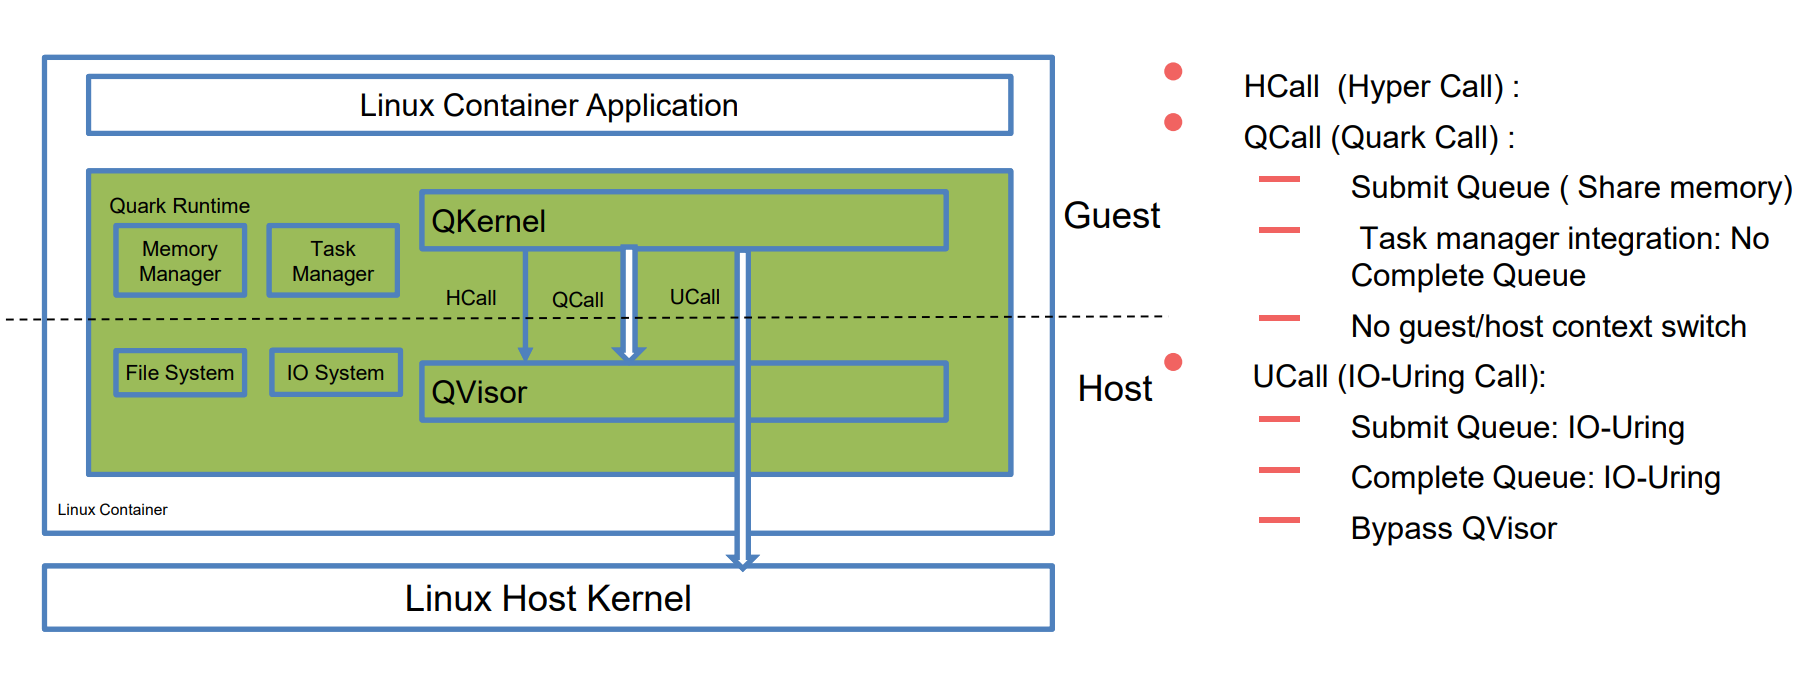
\includegraphics[width=0.8\textwidth]{images/quark_io.png}
    \caption[quark IO]{quark IO}
    \label{fig:quark_io}
\end{figure}

\todo{add long description for quark IO, modify the image: add Guest System Call btw. container app and qkernel}

\subsection{Qcall, Hypercall, and Ucall}
\label{Qcall_hypercall_ucall}
\begin{figure}[H]
  \centering
  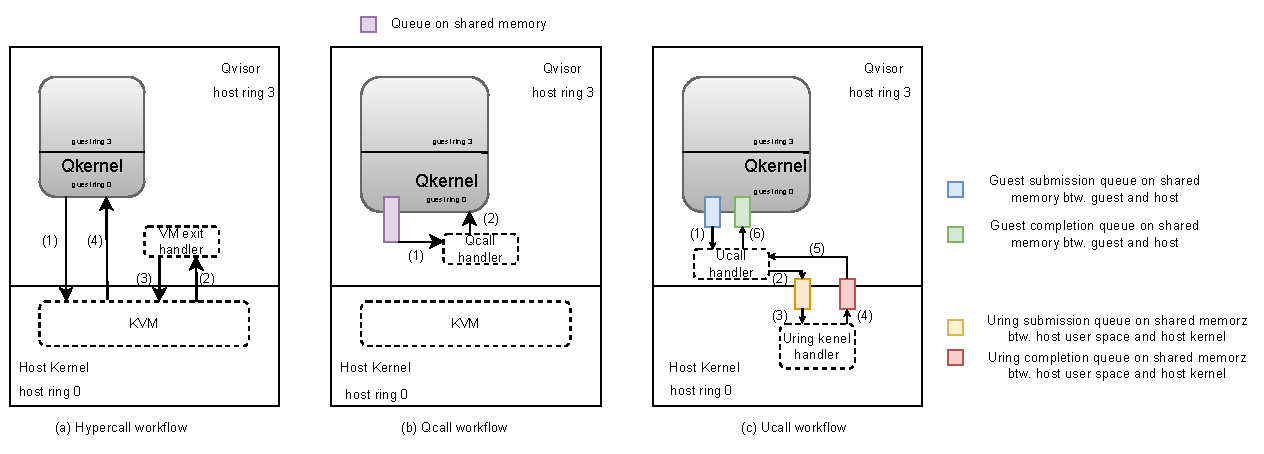
\includegraphics[width=0.8\textwidth]{images/hypercall_qcall_ucall.pdf}
  \caption[Workflow of Hypercall, Qcall, and Ucall]{Workflow of Hypercall, Qcall, and Ucall}
  \label{fig:hypercall_qcall_ucall}
\end{figure}
\todo{describe the workflow of Hypercall, Qcall, and Ucall in figure's long description}
Hypercall provides the qkernel with the means to issue commands to the Qvisor. Figure ~\ref{fig:hypercall_qcall_ucall}(a) shows the hypercall workflow in the context of Quark. 
When qkernel triggers a hypercall, the CPU leaves guest ring 0 mode and enters host ring 0 mode (~\ref{fig:hypercall_qcall_ucall}a (1)). KVM then checks the reason for the VM exit by examining the VMCB and forwards the 
hypercall to Qvisor running on host ring 3 mode (~\ref{fig:hypercall_qcall_ucall}a (2)). After handling the hypercall request, Qvisor invokes KVM, which resumes qkernel execution in guest ring 0 mode (~\ref{fig:hypercall_qcall_ucall}a (3), (4)).
With hypercall, the Qkernel can access service in Qvisor, such as opening a file, initializing IO. Unfortunately, 
this approach is very expensive due to the context switching between the Qkenel and Qvisor. 

To this end, Quark provides an asynchronous mechanism called Qcall as an alternative. 
As shown in Figure ~\ref{fig:hypercall_qcall_ucall}(b), this mechanism is implemented by a queue on shared memory between the Qkernel and the Qvisor and an io thread on the Qvisor side, where the
shared queue is used to transfer requests sent by the Qkernel to the Qvisor, and the io thread is responsible for retrieving requests from the queue and notifying the Qkernel thread when the Qivosr completes 
the request. Through this mechanism, Qkernel is able to access services in Qvisor in an asynchronous manner without VM exit, which improves the performance of the Qkernel significantly.

Typically, IO operations with hypercall are expensive. Therefore, Quark introduced the Ucall interface as a means of direct communication between the Qkernel and the host kernel for host 
IO data operations,  such as socket reading and writing. It supports both synchronous and asynchronous IO operations. Figure ~\ref{fig:hypercall_qcall_ucall}(c) details the workflow of the Qkernel 
using Ucall for synchronous IO operations. First, the qkernel thread submits the IO request into the guest submission queue (Figure ~\ref{fig:hypercall_qcall_ucall}c (1)). Then the Qvisor Ucall handler thread copies the request to the uring submission 
queue (Figure ~\ref{fig:hypercall_qcall_ucall}c (2)). After the Uring kernel hander finishes processing the IO request, it puts the IO processing result into the uring completion queue (Figure ~\ref{fig:hypercall_qcall_ucall}c (3), (4)). The result 
contains a user\_data field, which is submitted from the initial IO request and contains information about the Qkernel thread that submitted the IO request. By reading this field, the Qvisor Ucall handler thread wakes up the corresponding Qkernel thread 
after copying the IO processing result to the guest completion queue (Figure ~\ref{fig:hypercall_qcall_ucall}c (5), (6)).



\section{TEE --generic Idea}
The hardware-assisted Trusted Execution Environment (TEE) provides one or more tamper-proof computing environments that ensure data confidentiality and integrity. Such environment is also called enclave. It protects security-sensitive applications from co-located attackers 
through verifiable boot of the execution environment, CPU and memory isolation, trusted IO, and secure storage\cite*{Hardware-supported-TEE}. This security guarantee relays on specialized chips. Therefore, breaking various software layers,
such as operating systems and hypervisors, do not affect TEE's ability to protect sensitive computation and data\cite*{7345265}.

As shown in Figure ~\ref{fig:vm_process_tee}, hardware-based TEE models can be conceptually divided into two categories, namely VM-based TEE and process-based TEE\cite*{101145}. In VM-based TEE models, the entire VM memory is encrypted with a hardware-based encryption key to protect the VM from other privileged 
software components, such as hypervisor and operating system. Examples of VM-based TEE include AMD SEV\cite*{AMD_SEV}, INTEL TDX\cite*{Inte_TDX}, etc. On the other hand, process-based TEE encrypts only a segment of memory in the application address space,  i.e., the address 
space is divided into two parts, a trusted region and an untrusted region, which communicate with each other through call gates. 
Examples of process-based TEE implementation 
are INTEL SGX\cite*{INTEL_SGX} and OpenPOWER's Sanctum\cite*{Costan2016SanctumMH}.
\begin{figure}[H]
  \centering
  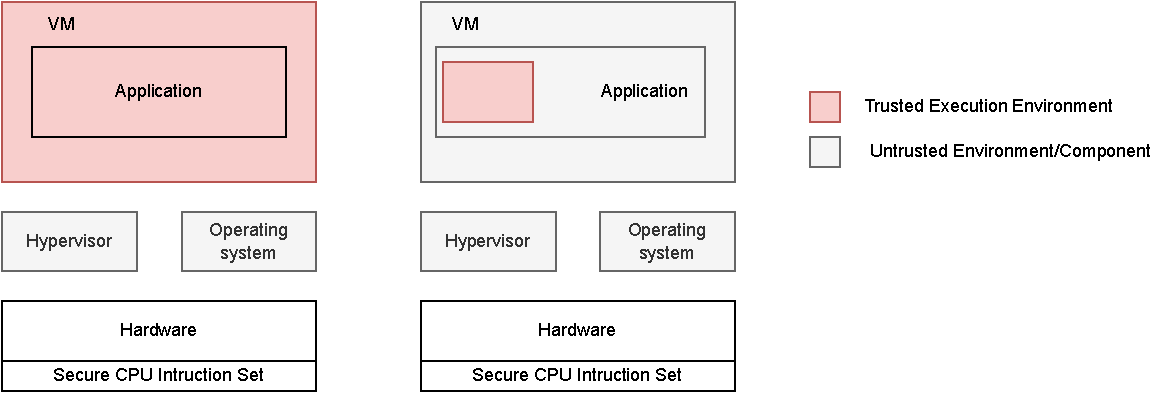
\includegraphics[width=0.8\textwidth]{images/vm_process_tee.pdf}
  \caption[VM based vs process based TEE model]{VM based vs process based TEE model}
  \label{fig:vm_process_tee}
\end{figure}

Both of these models have their advantages and disadvantages\cite*{10.3389/fcomp.2022.930741} \cite*{Execution_Environment_landscape} \cite*{101145}. Take Intel SGX as an example of process-based TEE. Compared to VM-based TEE, it has the advantage of a smaller TCB, i.e., a smaller attack surface. However, the disadvantages are also obvious. A frequently 
cited disadvantage is the need for significant software modifications to accommodate this TEE model. Other drawbacks include performance degradation due to limited EPC size in case a process requires a huge area of encrypted memory. Furthermore, this model 
may cause a significant performance penalty for IO-intensive applications, as it only allows enclave to perform system calls and hardware accesses via Ocall and Ecall, which can be very expensive.


The VM-based approach has the following advantages. First, it provides bi-directional isolation, alleviating the concern about malware running in the enclave corrupting the other components on the same host. In addition, it is more 
flexible compared to process base approaches as it supports running security-sensitive programs in an enclave (VM) without modification. However, placing the entire virtual machine under the protection of the TEE increases the TCB, making the approach more vulnerable to attacks.


In the next two sections, we describe in more detail how VM-based TEE safeguards sensitive data by means of memory encryption, attestation, etc. We choose AMD SEV and INTEL TDX as examples and compare their differences since they may be widely used by the industry in the future.
Also, since our implementation is based on VM-based TEE, 
a detailed description of process-based TEE is considered out of the scope. For a detailed explanation of process-based TEE, we refer the reader to \cite*{cryptoeprint:2016/086} \cite*{10.1145/2487726.2488370} \cite*{SGX_PAPER_LIST}.


\subsection{AMD SEV SNP}
AMD SEV SNP\cite*{sev_smp} is AMD's latest virtual machine-based TEE solution. It retains the features of its predecessor (AMD SEV\cite*{sev} and AMD SEV-ES\cite*{sev_es}), namely VM memory 
encryption, register state protection after VM exit, and further adds integrity protection for encrypted memory.

AMD SEV SNP protects the virtual machine's memory with encryption. When a service running in an enclave (VM) accesses memory, the AES-128 encryption engine embedded in the memory controller 
transparently encrypts or decrypts the memory using a memory encryption key. Note that each enclave is assigned a unique memory encryption, and this key will never be revealed to an untrusted 
entity, such as a hypervisor. As a result, untrusted entities can only read the cipher text on the VM's memory. To enable sharing of memory pages between enclaves or between an enclave and 
hypervisor, a new control bit, the "C-bit," is introduced in the page table entry, allowing the enclave to decide which page should be encrypted.

To mitigate attacks on VM control blocks during VM exits, SNP supports non-automatic VM exits. SNP classifies VM exits into two categories: automatic VM exits and non-automatic VM exits. 
Automatic VM exits refer to VM exits that do not expose any guest register state to the hypervisor. Examples of automatic VM exits include those triggered by physical interrupts, shutdowns, 
and the hlt instruction, etc. All other exits are non-automatic VM exits, i.e., exits of VMs that require exposing the state of the guest registers to the hypervisor. In this case, 
SNP allows the guest to select the registers that need to be exposed to the hypervisor and encrypt the remaining register state before the VM exits.

In comparison to its predecessor, AMD SNP protects the integrity of enclave memory by introducing Reverse Map Tabel (RMP), which helps SNP enforce the ownership of a physical page to one entity, i.e., 
only the owner of a page can modify that page. In addition, changing the ownership of a page will erase the contents of that page. In this way, malicious entities may only read the 
encrypted virtual machine memory rather than modify it.

SEV SNP also supports attestation. It allows the secret owner to verify the trustworthiness of the enclave and decide whether to make the secrets in their possession available to the enclave. 
This process is also referred to as attestation and provisioning. Compared to its predecessors, AMD SEV, and AMD SEV-ES, SNP not only retains the static attestation, i.e., the attestation during 
enclave launch, but also adds the runtime attestation feature. This feature makes the SNP's attestation more flexible as it allows the verifier to examine the trustworthiness of the enclave at 
any time while it is running. It is also interesting to note that the AMD SEV family does not support local attestation compared to intel's TEE solutions. As such, this section skips the 
explanation of local attestation. For those interested in local attestation, please refer to the next section on Intel TDX \ref*{subsec:tdx}.

Remote attestation for SEV SNP relies on three keys, the  Chip Endorsement Key (CEK), the e AMD SEV Signing Key (ASK), and the AMD root signing key(RSK), to establish 
the root of trust\cite*{Menetrey2022AnES}. CEK is a P-384 ECDSA chip-unique signing key fused into the processor die, while ASK and ARK are global keys securely stored by AMD. The relationship between these three 
keys is that CEK on each AMD platform is signed by ASK, and ASK is signed by ARK. During the runtime of the enclave, the certifier can request an attestation report signed by the CEK from the enclave. 
This report contains measurements related to the enclave, which include measurements on the contents of the enclave memory, the configuration of the platform on which the enclave is running, etc.
 In addition, the report includes a 512-bit custom guest data field to, for example, prove freshness to the verifier or establish a mutual TLS communication channel between the enclave and the 
 verifier. In the end, after obtaining the report, the verifier can verify the report using the public key of the AMD signature key obtained from AMD and decide whether the enclave should be 
 provisioned based on the measurements in the report.

\subsection{Intel TDX}
\label{subsec:tdx}

Intel has also announced its virtual machine-based solution called Intel TDX\cite*{Intel_tdx_whitepaper}. Although TDX has yet to be available to the market, several system-level software\cite*{Kate_support_tdx} \cite*{Linux_support_tdx}, including our implementation, 
have already decided to adopt Intel TDX. Hence we decided to give a brief introduction to INTEL TDX. 

Figure ~\ref{fig:TDX_diagram} illustrates The Architecture of Intel TDX. All trust domains (TDs), as well as the digitally signed TDX module, run in a new CPU mode, i.e.,  "Secure Arbitration Mode (SEAM)."
This new mode offers an isolated execution environment for TDs so that privileged software running in other modes (hypervisor, operating system, etc.) cannot eavesdrop on the TD's state, including 
register states, memory contents, etc.   The TDX module running in SEAM root mode is responsible for running TDs in SEAM guest mode and offers an interface for host-side VMM to 
manage the TDs. This interface enables the TDX module to validate commands to TDs issued by VMM and enforce security policies around those commands with the aim of keeping the data confidentiality 
and integrity inside TDs. 
\begin{figure}[H]
  \centering
  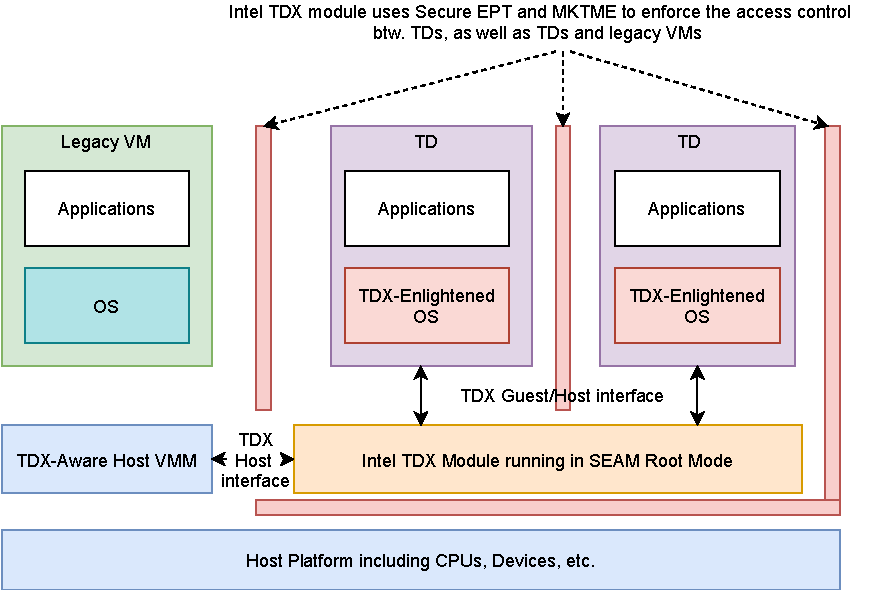
\includegraphics[width=0.8\textwidth]{images/TDX_diagram.pdf}
  \caption[Intel TDX model]{Intel TDX model}
  \label{fig:TDX_diagram}
\end{figure}
\todo{add reference to this figure}
Intel TDX offers confidentiality and integrity of memory and CPU state to TDs. This is achieved by reusing a so-called multi-key, total-memory-encryption engine 
(MKTME), which provides encryption using AES-128-XTS, integrity using 28-bit MAC, and a TD-ownership bit associated with each cache line\cite*{Intel_tdx_whitepaper}. Under the hood, the 
MKTME in the memory controller performs memory encryption to each TD using a TD-assigned private key. Such keys are managed by the TDX model in SEAM mode and are 
not accessible by the hypervisor. Furthermore, TDX leverages the TD-ownership bit to determine if a cache line is tied with a page assigned to a TD. In case an 
entity does not possess the right memory encryption key and tries to access memory with this bit set, the entity can only get a dummy value\cite*{Intel_tdx_whitepaper}. In this way, we 
effectively avoid ciphertext analysis. Last but not least, MAC associated with each memory line provide  TDX with a way to detect state tamper for encrypted memory.   
And cause a TD to terminate if a MAC violation happens.

TDX also supports shared memory to facilitate TD communication with untrusted external entities. Unlike the private memory of a TD that is protected by cryptographic encryption and SHA-3-based MAC 
using the TD-assigned private key, external entities such as hypervisors can access the shared memory in plain text. This mechanism is achieved by introducing a new bit called "Shared Bit" 
on TD's page table entry (guest page table entry) and  2 EPTs, namely a secure EPT and a shared EPT. TD leverage this shared bit to determine if a GPA maps to shared memory. The secure EPT and 
the shared EPT are used to translate the private/shared GPA to the physical address, respectively. Besides, the Intel-TDX module hosts a data structure called Physical-Address-Metadata Tabe to 
enforce page ownership. In this way, a page cannot be mapped to two TD's secure EPT at the same time.

TDX is designed to offer local and remote attestation by reusing and extending the attestation infrastructure from Intel SGX\cite*{Intel_tdx_whitepaper}, e.g., quoting enclave, Intel SGX DCAP. One principle difference is 
that the local attestation verifier and challenger reside on the same host, and the root of trust is built upon the shared platform hardware, while building the root of trust in remote attestation 
requires a more sophisticated solution, like DCAP\cite*{Intel_DCAP}, or EPID\cite*{Intel_EPID}.   

In the Intel TDX local attestation, a new instruction is provided to generate the local report for the attester (TD). This local report includes the measurement associated with a TD (hash value), 
SVNs of TDX-TCB elements, and customized data from the TD\cite*{Intel_tdx_whitepaper}. Furthermore, this report is integrity-protected and cryptographically tied to the hardware shared between the verifier and the attester 
using a message authentication code (MAC). Thus, the verifier can then use EVERIFYREPORT instructions to verify this report and determine the trustworthiness of the attester. 

 
The root of trust for Intel TDX remote attestation is offered by a certification infrastructure that reuses the Intel sgx DCAP\cite*{Intel_DCAP} and quoting enclave\cite*{Intel_tdx_whitepaper}. Quoting enclave shares the same hardware 
platform with the attester (TD) and is responsible for generating a quote for a local attestation report after verifying the report. Quoting enclave on the same hardware platform with the 
attester (TD) is responsible for generating a quote for a local attestation report after verifying the report using EVERIFYREPORT instructions. This quote is digitally signed by an 
attestation key owned by quoting enclave, and the remote verifier can verify it by consulting the Intel certification authority. For the detailed explanation of the Intel TDX remote attestation, we refer the reader to \cite*{Intel_tdx_whitepaper}, \cite*{9448036}.


\subsection{KBS Attestation Protocol}

We use the Key Broke service attestation protocol to establish a communication channel between a Key Broke client (KBC) and a trusted Key Broker Service (KBS), 
through which the KBS can verify that the KBC is running in a trusted environment and inject secrets into the KBC in a secure manner. It allows KBS to attest against KBC in a Request-Challenge-Attestation-Response (RCAR) manner and subsequently insect secrets to KBC securely. 
To facilitate the authentication of the KBS identity by the KBC and to prevent rogue attackers from hijacking the KBS address to spoof the KBC, the protocol uses HTTPS. More specifically, the protocol requires that the public key of the KBS be distributed to the KBC in an efficient manner so that 
the KBC can authenticate the KBS identity during the tls handshake later on.  Note that in our context, the KBC is the confidential qkernel, while the CAS is the key broker service.

The protocol is divided into two phases. In the first phase (authentication phase), the KBS authenticates the KBC by requiring the attestation report from it. In the second phase (Resource Requests phase), KBS allow KBCs to request protected resources from it. 
KBS uses the public part of an asymmetric key received from KBC in the first phase to encrypt the secret of the KBC request. Notice that the hash of this key is included in attestation report of the KBC and signed by the HW-TEE. Therefore, KBS 
can confirm that the key comes from the KBC and only the KBC can decrypt the encrypted secret. For performance degradation due to multiple attestations in case the KBC requires multiple resources, resulting in multiple requests to the KBS, 
it uses the standard HTTP cookie mechanism.  Since the HTTP cookie binds the authentication result of phase one, KBC can request secrets from KBS within the valid time of the HTTP cookie without having to go through the authentication phase again.

The following 2 diagrams detail how KBS and KBC work in stages 1 and 2 in order to complete the secret provisioning in an effective and secure fashion.
\begin{figure}[H]
    \centering
    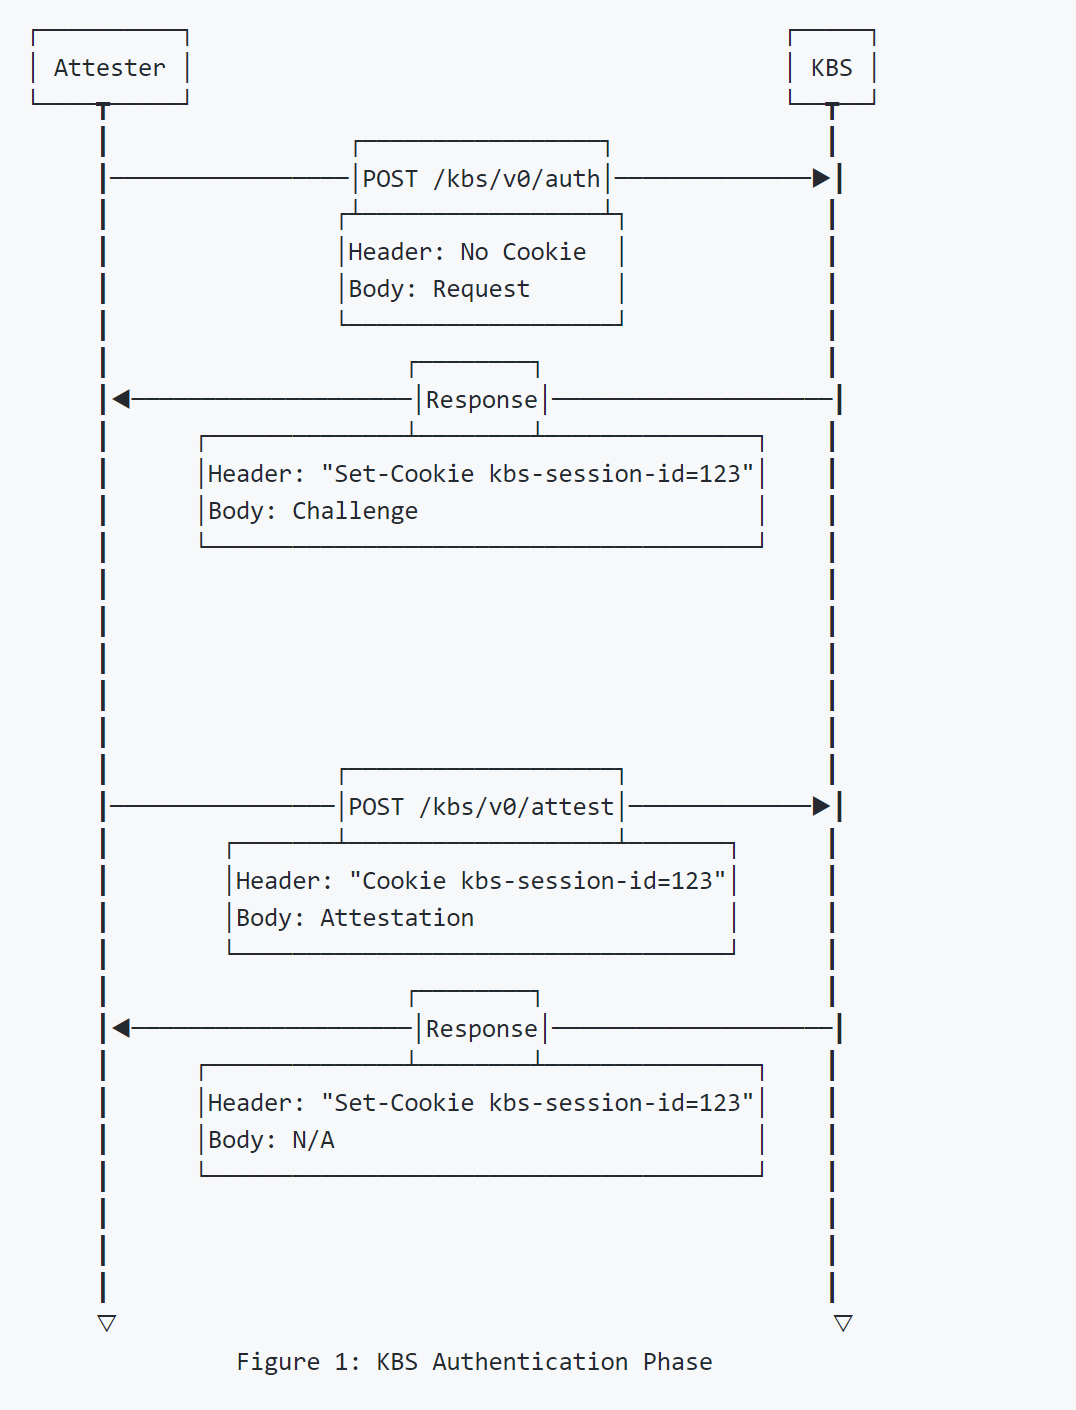
\includegraphics[width=0.8\textwidth]{images/attestation.PNG}
    \caption[Authentication phase]{Authentication phase}
    \label{fig:Authentication}
\end{figure}

As defined in Key Broke service attestation protocol, phase 1 (authentication phase) has 4 step: 
\begin{displayquote}
    \begin{enumerate}
        \item  Request: The KBC sends the initial Request payload to the KBS, in order to authenticate itself against the KBS, and eventually request resources.
        \item  Challenge: After receiving the initial Request payload, the KBS responds with the Challenge payload. This is how the KBS sends the attestation challenge to the KBC. Together with the attestation challenge, the KBS also sends a session identifier to the KBC, as an HTTP Cookie. This session identifier can be used to skip steps 2 and 3 after a successful attestation.
        \item  Attestation: The KBC replies to the attestation challenge from step 2 with an attestation evidence, in order to prove that its environment (HW-TEE) is safe and reliable. The KBC sends an Attestation payload to the KBS, that contains the attestation evidence and the HW-TEE generated, ephemeral public key.
        \item  Response: The KBS returns a Response payload to a KBC requesting a resource if and only if the Attestation payload was successfully validated. The KBC requests resources by sending HTTP GET requests to resource specific endpoints. Within the valid time of the HTTP Cookie generated by the KBS during step 2, the KBC can directly request resources or services from KBS, without going through steps 2 and 3.
    \end{enumerate}
\end{displayquote}

\begin{figure}[H]
    \centering
    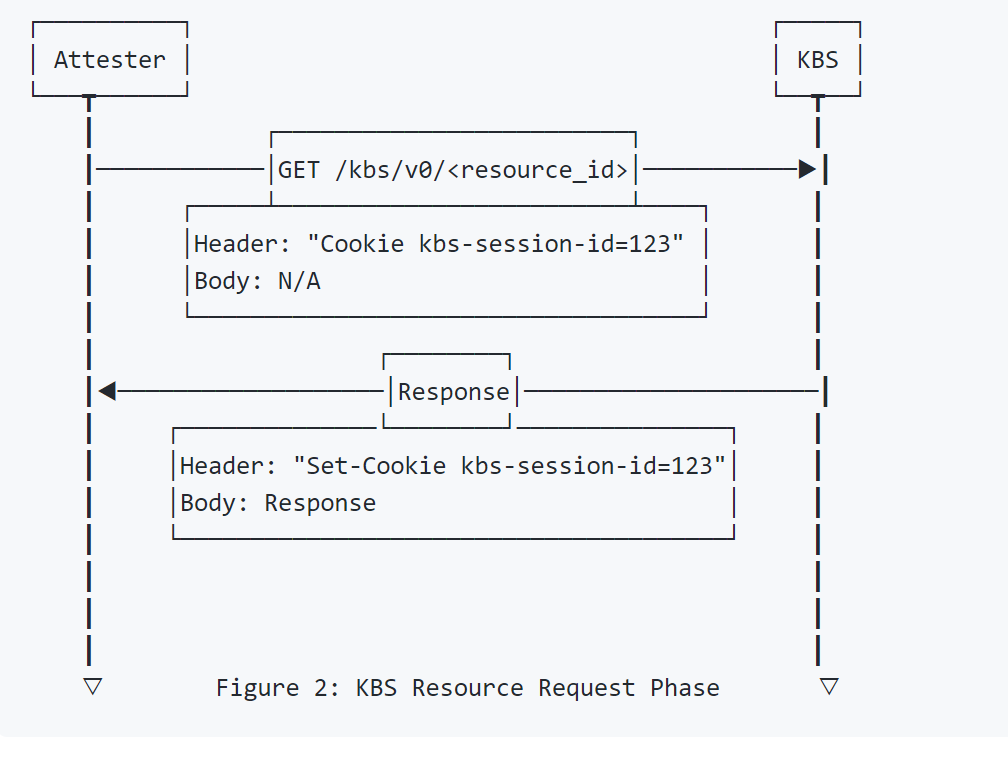
\includegraphics[width=0.8\textwidth]{images/resourcerequrie.PNG}
    \caption[Resource Requests phase]{Resource Requests phase}
    \label{fig:resourcerequrie}
\end{figure}
As defined in Key Broke service attestation protocol,  kbc can request resources or services from kbs during 2 phase in the following way:
\begin{displayquote}
    The KBS implementation keeps track of attestation results and binds them to a cookie identifier. During the second phase, the KBS can then decide if a specific resource could be released to a given attester, by mapping the cookie identifier the attester includes in 
    its resource request message to its attestation results.

    To request a protected resource from the KBS, the attester sends a GET request to a resource specific endpoint. If the attester is allowed to access the resource, the KBS will respond to the 
    GET request with an HTTP response which content is set to a KBS Response JSON payload.
\end{displayquote}




\section{ACCESS CONTROL}

\section{Summary}
In this chapter, I first give an overview of the various components of k8s and two standards that make k8s more extensible. Furthermore, I depict the general architecture of the quark container 
and the interfaces that qkernel used to communicate with qvisor and host kernel. Last but not least, I describe the concepts related to TEE, such as memory protection, attestation.

\cleardoublepage

%%% Local Variables:
%%% TeX-master: "diplom"
%%% End:
